\chapter{Editing}
There are three types of objects which can be exported to a MDL: Empties,
Meshes and Lamps. Other objects like curves and surfaces will have to be
converted to meshes before attempting to export them.

\section{Empties}
Empties appear in MDLs as Dummies. Like in Blender they are used to group
objects. In addition there are special types of Empties/Dummies which for
example indicate locations for effects.

\subsection{Aurora Root}
Each MDL requires at least one Empty: The Aurora Root or Rootdummy. It holds 
additional information and indicates which objects belong to an MDL. All children
of a single Rootdummy are considered to be part of the same MDL. \\

An Empty without a parent is automatically considered a Rootdummy. 
The Rootdummy must have the same name as the MDL file (minus the file extension). \\

A Rootdummy has the following properties:
\subsubsection*{Classification}
\begin{description}[leftmargin=6em,style=nextline]
    \item[Item] Any inventory item.
    \item[GUI] Unknown.
    \item[Effect] For visual effects.
    \item[Door] Doors, be it generic or for tilesets.
    \item[Character] Creature or placeables. 
    \item[Tile] For tilesets.
    \item[Unknown] Avoid using this. It may be set during import.
\end{description}

\subsubsection*{Supermodel}
Reference to another MDL file. All animations from that file 
will be available in this MDL.

\subsubsection*{Animationscale}
Unknown

\subsection{Dummy}
Simple Empties with a parent are either used to group objects or
indicate a special location to the engine. \\

\begin{figure}
  \centering
  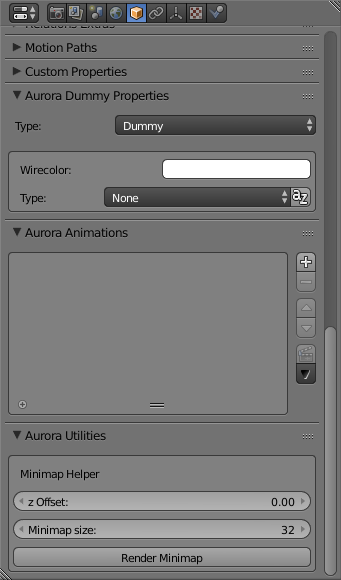
\includegraphics[trim=0 0 0 0, clip, width=0.33\textwidth]{panel_dummy}
  \caption[panel dummy]{Dummy Property Panel}
  \label{fig:panel_dummy}
\end{figure}

The following types of Dummies are available:
\begin{description}[leftmargin=6em,style=nextline]
    \item[None] Simple dummy without any special purpose.
    \item[Ground] Indicates the ground level for spells/ visual effects
    \item[Impact] Impact target for most spells/ visual effects.
    \item[Head Hit] Spells/ visual effects
    \item[Head] Head location for Spells/ visual effects
    \item[Hand] Point of origin for (some) spells. If a spell/ visual is originating from this mdl, this will be the point of origin most of the time.
    \item[Use 1] Use Node for placeables or doors. Upon receiving a use command a character will move to the closest of the two use nodes.
    \item[Use 2] Use Node for placeables or doors. Upon receiving a use command a character will move to the closest of the two use nodes.
\end{description}
None of the special Dummies are mandatory. If one is
missing from the MDL, the engine will use (0,0,0) as the default location
for that particular Dummy. \\

Selecting the type is not enough to make a Dummy work, they need to have
the correct name or to be precise: The correct suffix.
The export script will try to generate a valid name depending on
the Dummy's type, but it is recommended to do it manually to avoid naming
conflicts. \\

Use the button next to the Dummytype selector to generate a
working name. The Rootdummy's name will be used to create a working
suffix for the selected Dummytype. \\

\subsection{Reference Node}
The purpose and usage of these nodes is unknown. Supposedly it can be used to
reference other MDL files. These nodes can be found in some visual effects and reference fx\_ref 
most of the time.

\subsection{Patch Node}
The purpose and usage of these nodes is unknown. They occur in some visual effects, but
they seem to behave exactly like normal dummy nodes, i.e they have the same
attributes.

\section{Meshes}

\subsection{Trimeshes}
The default type of mesh for an MDL. As the name suggests it consisting of 
triangles, but it is unnecessary to explicitly convert the faces to triangles 
as Neverblender does that automatically during the export process.

\subsubsection*{Wirecolor}
This property is unused by the engine. It can safely be ignored. It probably defines the
color for the object's wire-frame in 3dsmax and exists in Neverblender only for 
compatibility reasons.

\subsubsection*{Self-Illumination Color}
Makes the mesh seem to glow. It does not act as a light source however.
This property will not be displayed in blender's viewports or renderers.

\subsubsection*{Ambient Color}
OpenGL material property. The engine uses per-object ambient light whereas Blender's 
defines it on a per scene basis. Therefore this property is not displayed in 
Blender's viewports or renderers.

\subsubsection*{Shininess}
Shininess requires a matching .txi file for the texture and a .env file.

\subsubsection*{Tilefade}
This property is only relevant for tiles. It controls whether this 
mesh will turn invisible to clear the view.
\begin{description}[leftmargin=6em,style=nextline]
    \item[None] This mesh will always be visible.
    \item[Fade] The object will fade.
    \item[Base] Unknown
    \item[Neighbour] The object will fade along with meshes in neighbouring tiles.
\end{description}

\subsubsection*{Render}
This property controls whether this object should be rendered. Note: Meshes can still
cast a shadow without being rendered.

\subsubsection*{Shadow}
Controls whether this objects should cast a shadow. 

Trimeshes with disabled rendering and enabled shadows are also called Shadowmeshes.
It is recommended to disable Shadows for complex Meshes with a 
large amount of triangles and use a Shadowmesh with a low polycount instead. 
Failing to do so might negatively impact performance and corrupt the shadows of the 
model as the engine is only capable of handling shadows for simple, convex objects.

\subsubsection*{Beaming}
Unknown. Probably unused.

\subsubsection*{Inherit Color}
Unknown. Probably unused.

\subsubsection*{Rotatetexture}
Only available for tiles. Auto-Rotates textures so the UVs are rotated
the same way to avoids seams between tiles.

\subsubsection*{Transparencyhint}
This helps the engine prioritize transparent meshes, similar to a z-buffer.
Multiple overlapping meshes with transparency can cause issues like
flickering, which may be resolved by changing this property.

\subsubsection*{Smoothgroup}
Controls how or whether at all to create smoothing groups or shading groups.
\begin{description}[leftmargin=6em,style=nextline]
    \item[Separate] Each face will have its own smoothing group. This results in no smoothing at all.
    \item[Single] All faces belong to a single smoothing group. Meshes will be smoothed completely.
    \item[Auto] Auto generate smoothing groups, depending on the settings in blender and edges marked as sharp. Replicates blenders smoothing as closely as possible.
\end{description}

\subsection{Danglymeshes}
Danglymeshes are Trimeshes which are "bouncy" or "dangly". They are affected by
wind, character movement and visual effects. A set of weights determine how far a 
vertex can be displaced from its original position.

A Danglymesh has the following properties in addition to the properties of a 
trimesh:
\begin{description}[leftmargin=6em,style=nextline]
    \item[Dangle group] The dangle group is a vertex group containing the weights of vertices for the danglymesh. You must select an existing vertex group.
    \item[Period]
    \item[Tightness]
    \item[Displacement]
\end{description}

\subsection{Skinmeshes}
A skinmesh is used to create skeletal animations. At the moment it is not 
possible to use Blender's armature system directly. Instead several vertex groups 
must be created with their names matching one of the other trimeshes in the MDL. 
Unfortunately this means that no animations are visible in blender which can make 
creation of new skinmeshes rather difficult.


\subsection{Animeshes}
Animeshes are Trimeshes with animated UV textures. At the moment Animeshes
are imported as Trimeshes and will thus lose their animations.


\subsection{Walkmeshes}
Walkmeshes indicate where a character can walk. It is necessary to select 
the appropriate type of walkmesh, which depends on the type of model itself. 
The following types are available:
\begin{description}[leftmargin=10em,style=nextline]
    \item[Tileset] Walkmesh for tiles. Assign Materials to each face to set the
                   surface type of tile (stone, grass, unwalkable, ...).
                   This will also affect footstep sounds and grass growth.
    \item[Door: Closed] The walkmesh for the closed state of a door. Blocks movement.
    \item[Door: Open 1] The Walkmesh for the first open state of a door. Blocks movement.
    \item[Door: Open 2] The Walkmesh for the second open state of a door. Blocks movement.
    \item[Placeable] Walkmesh for placeables. Blocks movement.
\end{description}
It is recommended to keep walkmeshes as simple as possible.

\section{Emitters}
Support for Emitters is rudimentary. Blenders particle systems is too
different to allow a direct import, instead Emitters are imported as plain
text. While all data will be retained, editing is difficult.

\section{Lamps}
Blender lamp properties will be used for exporting a light.
Exported properties are:
\begin{itemize}
\item Color
\item Distance
\end{itemize}

\subsection*{Light type}
There are some special light types, all of which are used to give builders
the ability to select light color in the Toolset.
\begin{description}[leftmargin=8em,style=nextline]
    \item[Mainlight 1] For Tiles only. Color can be changed in the Toolset.
    \item[Mainlight 2] For Tiles only. Color can be changed in the Toolset.
    \item[Sourcelight 1] For Tiles only. This is actually a burning flame. Color can be changed in the Toolset.
    \item[Sourcelight 2] For Tiles only. This is actually a burning flame. Color can be changed in the Toolset.
    \item[Default] Default type, can always be used. Blenders lamp properties will be used (color and distance)
\end{description}

\subsection*{Wirecolor}
This is unused in-game. You can safely ignore it. This probably defines the
color for the object's wireframe in 3dsmax.

\subsection*{Priority}
Unknown. Might control when the light source casts a shadow.

\subsection*{Ambient Only}
This controls if the light is only an ambient light source or
if it is directional as well.

\subsection*{Fading}
Unknown. Might activate some kind of distance fall off for the light.

\subsection*{Shadows}
Determines if this light is capable of casting shadows.

\subsection*{Is Dynamic}
Unknown.

\subsection*{Affect Dynamic}
This controls whether this light affects dynamic objects, i.e. characters.
Disabling this will prevent this light from casting shadows with dynamic
objects, but it will in turn improve performance.

This is basically a less strict version of the \textit{Shadows} setting.

\subsection*{Lensflares}
Add a series of lens-flares for this light.

Lens-flares are unavailable for Mainlights or Sourcelights.
\begin{description}[leftmargin=6em,style=nextline]
    \item[Texture] Texture for this flare
    \item[Colorshift] Unknown. Possibly color difference from the light color.
    \item[Size] Size of the flares. This will scale the texture.
    \item[Position] Distance from the lights origin.
\end{description}

\section{Materials \& Textures}
MDL files support a single material with a single texture. If multiple 
materials or textures are assigned, the export script will choose the currently 
active one or, failing that, the topmost one.

The following properties are exported:
\begin{itemize}
    \item Diffuse
    \item Specular
    \item Alpha values
\end{itemize}

\subsection*{Alpha}
Neverblender can export either material or texture alpha. When both properties are present 
the latter takes precedence.

\section{Animations}
Each animation has to be defined by name and start/end frames. Valid names 
are listed in the reference chapter for each type of MDL.

The following properties can be animated:
\begin{itemize}
    \item Location
    \item Rotation
    \item Scale (Uniform only)
    \item Material or Texture Alpha
    \item Self-Illumination color
    \item Lamp color
    \item Lamp distance (Light radius)
\end{itemize}
Animation data like start/end frames and name are stored in the Rootdummy. Deleting the Rootdummy will result in
the loss of this data.